\chapter{Background and Related Work Analysis}\label{bg}
In this Chapter we provide the reader with a review of the basic knowledge in fields of optimization problems and approaches for solving them.
A reader, experienced in field of optimization and search problems, may consider this chapter as an obvious discussion of well-known facts. 
If such notions as a \textit{parameter tuning} and a \textit{parameter control} are not familiar to you or seems the same, we highly encourage you to spend some time reading this chapter carefully.
In any case, it is worth for everyone to refresh the knowledge with coarse-grained description of topics, mentioned in this section and examine the examples of hyper-heuristics in \cref{bg: hh examples} and systems for parameter tuning in \cref{bg: parameter tuning expamples}.

The structure of this Chapter is defined as follows. Firstly, we give an informal definition of optimization problem and enumerate possible solver types in \cref{bg:section problems and solvers}. Secondly, we pay attention to the heuristic solvers, their weak points and \emph{No Free Lunch Theorem} in \cref{bg: section heuristics}. Afterwards, in \cref{bg: section Parameters Setting} we discuss the influence of parameter setting and possible approaches to set the parameters. \cref{bg: section cash}, dedicated to \emph{Combined Algorithm Selection and Hyper-parameter Tuning} problem, is followed by conclusion on the literature analysis outlining the thesis' scope in \cref{bg: conclusion}.

\section{Optimization Problems and their Solvers}\label{bg:section problems and solvers}
Our life is full of different difficult and sometimes contradicting choices. Optimization is an art of making good decisions.

A decision between working hard or going home earlier, to buy cheaper goods or to follow brands, to isolate ourselves or to visit friends during the quarantine, to spend more time for planning trip or to start it instantly. Each decision that we make, has its consequences.

\cref{bg:pic:Optimization tradeoff} outlines the trade-off between a decision quality and an amount of effort spent. The underlying idea of the research in optimization problems solving sphere is to squash this curve simultaneously down and to the left thus, deriving a better result with less cost when solving the optimization problem.

\svgpath{{graphics/Background/}}
\begin{figure}
	\centering
	\includesvg[width=0.7\textwidth]{optimization_concept}
	\caption{Optimization trade-off.}
	\label{bg:pic:Optimization tradeoff}
\end{figure}
\todoy{axes labels should be distinguishable from axes values (Dima review)}

\subsection{Optimization Problems}\label{BG: subsection OPs}
While the \emph{search problem} (SP) defines the process of finding a possible solution for the \emph{computation problem}, the \emph{optimization problem} (OP) defined as a special case of the SP, focused on the process of finding the \emph{best possible} solution for computation problem~\cite{goldreich2010p}.

The focus of this thesis is the optimization problems.

Most studies conducted in this field have tried to formalize the OP concept, but the underlying notion is so vast that it is hard to exclude the application domain from the definition. The description of every possible optimization problem and all approaches to its solving are not in the scope of this thesis, while we consider it necessary to present a coarse-grained review in order to make sure that readers are familiar with all the terms and notions mentioned in the thesis. 

To begin with, let us define the optimization \emph{subject}. Analytically, it could be represented as the function $Y = f(X)$ that accepts some input $X$ and reacts to it, providing an output $Y$. Informally, it could be imagined as the \emph{target system} $f$ (TS), shown on \cref{bg:pic:Target System}. It accepts the input information with its \emph{inputs} $X_n$, which are sometimes called variables or parameters, processes them performing some \emph{task} and produces the result on its \emph{outputs} $Y_m$.

\begin{figure}[!h]
	\centering
	\includesvg[width=0.5\textwidth]{TargetSystem}
	\caption{Optimization Target System.}
	\label{bg:pic:Target System}
\end{figure}

Each (unique) pair of sets $X_n^i$ and respective $Y_m^i$ form the $Solution^i$ for computational problem.
All possible inputs $X^i$, where $i=1...N$ form the \emph{search space} of $N$ size, while all outcomes $Y^i$, where $i=1...M$ form an \emph{objective space} of $M$ size.

The solution is characterized by the \emph{objective value(s)} — a quantitative measure of TS performance that we want to minimize or maximize in the optimization problems. We could obtain those value(s) directly, by reading the output on $Y_m$, or indirectly, for instance, noting the wall clock time TS took to produce the output $Y^i$ for given~$X^i$. The solution objective value(s) form the \emph{object} of optimization. 
For the sake of simplicity we here use $Y_m$, \textit{outputs} or \textit{objectives} interchangeably as well as $X_n$, \textit{variables} or \textit{parameters}.

\todoy{figure for classification}
Next, let us highlight the target system characteristics. In works~\cite{biegler2004retrospective,figueira2014hybrid,deb2014multi,amaran2016simulation} dedicated to solving the OPs, the authors distinguished OP characteristics that overlap through each of these works. Among them, we found the following properties to be the most important ones:
\begin{itemize}
	\item \textbf{Input data type} of $X_m$, which is a crucial characteristic. All input variables could be (1) \emph{discrete}, where representatives are binary strings, integer-ordered, or categorical data, (2) \emph{continuous}, where variables are usually a range of real numbers, or (3) \emph{mixed}, as the mixture of the previous two cases.

	\item \textbf{Constraints}, which describe the relationships among inputs and explain the dependencies in allowable values for them. As an example, imagine that having $X_n$ equal to $value$ implies that $X_{n + k}$ should not appear at all, or could take only some subset of all possible values.
	
	\item \textbf{Type of target system}, which is an amount of exposed knowledge about the dependencies $X \rightarrow Y$ before the optimization process starts. Taking this into consideration, an optimization could be of several types: \emph{white box} — it is possible to derive the algebraic model of TS, \emph{gray box} — the amount of exposed knowledge is significant, but not enough to build the algebraic model and \emph{black box} — the exposed knowledge is mostly negligible.
	%In this case the Derivative Free Optimization approaches (such as Surrogate Optimization, different Meta-|Hybrid-|Hyper-Heuristics)  are applicable.
	% http://downloads.hindawi.com/journals/mpe/2015/647234.pdf

	%\paragraph{Dependency types} could be  The inputs to outputs dependencies the of Target System could also be distinguished form perspective of linearity \cite{biegler2004retrospective,figueira2014hybrid}.
	%\textit{Linear dependencies} reveal the Linear Programming Optimization approaches, while with \textbf{Nonlinear dependencies} one should consider Nonlinear Programming.

	\item \textbf{Determinism of TS}, which is one of possible challenges, when the output is uncertain. TS is \emph{deterministic}, when it each time provides an equal output for the same input. However, in most real-life challenges engineers tackle \emph{stochastic} systems, the output of which is affected by random processes happened inside TS.

	\item \textbf{Cost of evaluation}, which is an amount of resources (energy, time, money, etc.) TS should spend to produce the output for particular input. It varies from \emph{cheap}, when TS could be an algebraic formula and task evaluation is a simple mathematic computation, to \emph{expensive}, when the TS is a pharmaceutical company, and the task is to perform a whole bunch of tests for a new drug, which may last years. 

	\item \textbf{Number of objectives}, which is a size of the output vector $Y_m^i$. With regard to this, the optimization could be either single- ($m=1$), or multi- ($m=2...M$) objective, where the result is one single solution, or a set of non-dominated (Pareto-optimal) solutions.
\end{itemize}

Most optimization problem types could be obtained by combining different types of each characteristic listed above.

In this thesis we tackle practical combinatorial problems, where the most prominent examples are \emph{bin packing}~\cite{martello1990bin}, \emph{job-shop scheduling}~\cite{blazewicz1996job} or \emph{vehicle routing}~\cite{toth2002vehicle} optimization problems.
All combinatorial problems are \emph{NP-Complete} meaning they are in both \emph{NP} and \emph{NP-Hard} complexity classes\cite{garey1979computers}. NP complexity implies that the solution is verifiable in the polynomial time, while in the NP-Hard case, the problem can be transformed to other NP-Complete problem in polynomial time, allowing to use a different solving algorithm.

As an example, let us grasp these characteristics for \emph{traveling salesman problem} (TSP)~\cite{applegate2006traveling} — an instance of the vehicle routing problem~\cite{laporte1992vehicle} and one of the most frequently studied a combinatorial OP (here we consider deterministic and symmetric TSP).
The informal definition of TSP is as follows: ``Given a set of $N$ cities and the distances between each of them, what is the shortest path that visits each city once and returns to the origin city?''
With respect to our previous definition of the optimization problem, the target system here is a function that evaluates the length of proposed path. The TSP distance (or cost) matrix is used in this function for the evaluation and it is clear that this TS exposes all internal knowledge therefore, it is a white box.
The input $X_n$ is a vector of city indexes as a result, the type of input data is non-negative integers. There are two constraints for the path: it should contain only unique indexes (visit each city only once) and it should start and end from the same city:~$[2 \rightarrow 1 \rightarrow ... \rightarrow 2]$.
Since the cost matrix is fixed and not changing during the solving process, the TS is considered to be deterministic and costs of two identical paths are always the same. Nevertheless, there exist Dynamic TSP where the cost matrix changes at runtime to reflect a more realistic real-time traffic updates\cite{cheong2011dynamic}.
It is cheap to compute a cost for a given path using the cost matrix therefore, overall solution evaluation in this OP is cheap, and $n = N!$ is the overall number of solutions. Since we are optimizing only the route distance, this is a single-objective OP.


\subsection{Optimization Problem Solvers}\label{BG: subsection OP Solvers}
Most of the optimization problems could be solved by an \emph{exhaustive search} — trying all possible combinations of the input variables and choosing the one, which provides the best objective value. This approach guarantees finding a globally optimal solution of the OP. But when the search space size significantly increases, the brute-force approach becomes infeasible and in many cases solving even the relatively small problem instances takes too much time.

Here, different optimization techniques come into play. Characteristics exposed by target system could restrict and sometimes strictly define the applicable approach.
For instance, imagine you have a white-box deterministic TS with a discrete constrained input data and a cheap evaluation. The OP in this case could be solved using the \emph{Integer Linear Programming} (ILP), or a heuristic approaches. But if this TS turned out to be a black-box, the ILP approaches will not be applicable anymore and one should consider using the heuristics~\cite{biegler2004retrospective}.

Evidently, there exist a lot of different facets for optimization problem solvers classification, but they are a subject of many surveying works~\cite{junger2003combinatorial,biegler2004retrospective,festa2014brief}. In this thesis, as the point of interest we highlight only two of them.

\begin{itemize}
	\item \textbf{Solution quality} perspective:
	\begin{enumerate}
		\item \textbf{Exact} solvers are those algorithms that always provide an optimal OP solution.
		\item \textbf{Approximate} solvers produce a sub-optimal output with guarantee in quality (some order of distance to the optimal solution).
		\item \textbf{Heuristics} solvers do not give any worst-case guarantee for the final result quality.
	\end{enumerate}
	
	\item \textbf{Solution availability} perspective:
	\begin{enumerate}
		\item \textbf{Completion} algorithms report the results only at the end of their run.
		\item \textbf{Anytime} algorithms are designed for stepwise solution improvement thus, could expose intermediate results.
	\end{enumerate}
\end{itemize}

Each of these algorithm characteristics provide their own advantages, having, however, their own disadvantages. For instance, if solution is not available at any time, one will not be able to control the optimization process. On the contrary, if it is available, the overall performance may decrease. 
If the latter features are more or less self-explanatory, the former require more detailed explanation.

\subsubsection{Solution Quality}
\paragraph{Exact Solvers.}
As was stated above, the exact algorithms are those, which always solve OP to guaranteed optimality. For some OP it is possible to develop an effective algorithm that is much faster than the exhaustive search — they run in a super-polynomial time, instead of exponential, still providing an optimal solution. As authors claimed in~\cite{woeginger2003exact}, if the common belief $P \ne NP$ is true, the super-polynomial time algorithms are the best we can hope to get when dealing with the NP-complete combinatorial problems.

According to the definition in~\cite{fomin2013exact}, the objective of an exact algorithm is to perform much better (in terms of running time) than the exhaustive search. In both works~\cite{woeginger2003exact,fomin2013exact} the authors enumerated main techniques for designing the exact algorithms. Each of these techniques contributes in this `better' independently and later they could be combined.

You may find a brief explanation of them below:
\begin{itemize}
	\item \textbf{Branching and bounding} techniques, when applied to the original problem, split the search space of all possible solutions (e.g. exhaustive enumeration) to a set of smaller sub-spaces. More formally, this process is called \emph{branching the search tree into sub-trees}. This is done with an intent to prove that some of sub-spaces never lead to an optimal solution and thus could be rejected.
	
	\item \textbf{Dynamic programming across sub-sets} technique could be combined with the  branching techniques. After forming the sub-trees, the dynamic programming attempts to derive the solutions for the smaller subsets and later combine them into the solutions for the lager subsets. This process repeats until the solution for original search space obtained.
	
	\item \textbf{Problem preprocessing} could be applied as an initial phase of the solving process. This technique is dependable upon the underlying OP, but when applied properly, significantly reduces the running time. A simple example from~\cite{woeginger2003exact} elegantly illustrates this technique: imagine a problem of finding a pair of two integers $x_i$ and $y_i$ in $X_k$ and $Y_k$ sets of unique numbers ($k$ here denotes the size of sets), that sum up to an integer $S$. The exhaustive search approach implies enumerating all $x-y$ pairs. The time complexity in this case is $O(k^2)$. But, if we firstly consider the data preprocessing by sorting and afterwards, using the bisection search repeatedly in these sorted arrays to find $k$ values $S - y_i$, then the overall time complexity reduces to $O(k\log(k))$.
\end{itemize}

\paragraph{Approximate Solvers.} When the OP cannot be solved to optimal in polynomial time, the only solution is to start thinking of the alternative ways to tackle it. A common decision is to apply the requirement \emph{relaxation techniques}~\cite{roubivcek2011relaxation} to derive the approximated solution.
Approximate algorithms are representatives of the theoretical computer science. They were created in order to tackle the computationally difficult (not solvable in super-polynomial time) white-box OP. Words of Garey and Johnson (computer scientists, authors of \textit{Computers and Intractability} book~\cite{garey1979computers}) could pay a perfect description of such approaches: ``I can't find an efficient algorithm, but neither can all of these famous people.''
%If the widely believed conjecture $P \ne NP$ is true, a wide range of OPs (ILP) are $NP-hard$ and cannot be solved with exact solvers in polynomial time, thus require relaxation either in efficiency or quality of optimization.

Unlike exact, approximate algorithms relax the quality requirements and solve the OP effectively with the provable assurances on the result distance from an optimal solution~\cite{williamson2011design}. The worst-case results quality guarantee is crucial in the approximation algorithms design and involves the mathematical proofs.

How do these algorithms guarantee on quality, if the optimal solution is unknown beforehand? — is a reasonable question arises at this point. Certainly, it sounds contradicting, but the comprehensive answer to this question requires an explanation of the key approximation algorithms design techniques that is not in the scope of this thesis. Nevertheless, let us briefly describe these techniques.

In~\cite{williamson2011design} the authors provided several techniques of the approximate solvers design. For instance, the \emph{Linear Programming} (LP) relaxation plays a central role in approximate solvers. It is well known, that solving the ILP is \textit{NP-hard} problem. However, it could be relaxed to the polynomial-time solvable linear programming. %Those, one of techniques is relaxation of ILP to LP. An optimal solution for LP will have value $S_LP \le S_IP = OPT$ (for the minimization case). Here we could derive a lower bound for the original minimization or upper bound for maximization problem. 
Later, a fractional solution for the LP will be rounded to obtain a feasible solution for the ILP. % that is within a cerain factor $f$ the value of the LP $S_LP$. Thus, the ILP solution will cost no more than $f * OPT$.
Different rounding strategies define separate approximate solver techniques~\cite{williamson2011design}: 
\begin{itemize}
	\item \textbf{Deterministic rounding} follows a predefined strategy.
	\item \textbf{Randomized rounding} performs a round-up of each fractional solution value to the integer uniformly.
\end{itemize}

In contrast to rounding, another technique requires building a \emph{Dual Linear Program} (DLP) for given linear program. This approach utilizes the \emph{weak} and \emph{strong duality} properties of DLP to derive the distance of the LP solution to the original ILP optimal solution. Other properties of DLP form a basis for the \emph{Primal-dual} algorithms. They start with a dual feasible solution and use the dual information to derive the primal linear program solution (possibly infeasible). If the primal solution is not feasible, the algorithm modifies the dual solution increasing the dual objective function values. In any case, these approaches are far beyond the thesis scope, but in case of an interest reader could start his own investigation from~\cite{williamson2011design}. 

\paragraph{Heuristics.} As opposed to the solvers mentioned above, heuristics do not provide any guarantee on the solution quality. They are applicable not only to the white-box TS, but also to the black-box cases. These approaches are sufficient to quickly reach an immediate, short-term goal in such cases, when the finding an optimal solution is impossible or impractical because of the huge search space size.

As in the reviewed above approaches, here exist many facets for classification.
We start from the largest one, namely the \textit{level of generality}:
\begin{itemize}
	\item \textbf{Simple heuristics} are the specifically designed to tackle the concrete problem algorithms. They fully rely on the domain knowledge, obtained from the optimization problem. Simple heuristics do not provide any mechanisms to escape a local optimum therefore, could be easily trapped to it~\cite{pearl1984intelligent}.
	
	\item \textbf{Meta-heuristics} are the high-level heuristics, that being domain knowledge dependent, also provide some level of generality to control the search. They could be applied to broader range of the OPs. They are often nature-inspired and comprise mechanisms to escape the local optima, but may converge slower than the simple heuristics. For the more detailed explanation we refer to survey~\cite{bianchi2009survey}.
	
	\item \textbf{Hybrid-heuristics} arise as the combinations of two or more meta-heuristics. They could be imagined as the recipes merge from the cook book, combining the best decisions to create something new and presumably better.
	
	\item \textbf{Hyper-heuristics} are the algorithms that operate in the search space of \emph{Low Level Heuristics} (LLH). Instead of tackling the original problem, they choose (or construct) LLHs, which will tackle this problem for them~\cite{burke2003hyper}. 
\end{itemize}

In the upcoming \cref{bg: section heuristics}, dedicated to heuristics, we provide more detailed information on each of the approaches mentioned above.


\subsubsection{The Most Suitable Solver Type}
\epigraph{``Fast, Cheap or Good? Choose two.''}{\textit{The old engineering slogan.}}

At this point, we have reached the crossroads and should make a decision, which way to follow.

Firstly, we have the exact solvers for the optimization problems. As mentioned above, they always guarantee to derive an optimal solution. Today, tomorrow, maybe in the next century, but eventually the exact solver will find it. The only thing we need is to construct the exact algorithm. This approach definitely offers the best final solution quality however, it sacrifices the solver construction simplicity and the speed in problem solving.

Secondly, we have the approximate solvers. They do not guarantee finding the one and only optimal solution, but suggest a provably good instead. From our perspective, the required effort for constructing the algorithm and proving its preciseness remains the same as for the exact solvers. However, this approach beats the previous one in the speed of problem solving, sacrificing a reasonably small amount of the result quality. It sounds like a good deal.

Finally, the remaining heuristic approaches. They quickly produce the solution, in comparison to the previous two. In addition, they are much easier to apply for the specific problem — there is no need to build a complex mathematical models or prove the theorems. However, the biggest flaw in these approaches is an absence of the solution quality guarantee therefore, one should consider them up to own risk.

As we mentioned in the \cref{BG: subsection OPs}, this thesis is dedicated to facing the practical combinatorial problems, such as the TSP. They are NP-complete, that is why we are not allowed to apply the exact solvers. In both approximate and heuristic solvers we are sacrificing the solution quality, though in different quantities. Nevertheless, the heuristic algorithms repay in the development time and provide the first results faster. The modern world is highly dynamic, in the business survive those, who are faster and stronger. In the most cases, former plays the crucial role for success. The great products are built iteratively, enhancing existing results step-by-step and leaving the unlucky decisions behind. It motivates us stick to the heuristic approach within the scope of the thesis.

In the following \cref{bg: section heuristics} we shortly survey different heuristic types and examples. We analyze their properties, weaknesses and ways to deal with them. As the result, we select the best suited class of heuristics for solving the TSP problem.

\section{Heuristic Solvers for Optimization Problems}\label{bg: section heuristics}
We base our descriptions of heuristics and their examples on the mentioned in \cref{BG: subsection OPs} traveling salesman problem. The input data $X$ to our heuristics will be the problem description in form of distance matrix (or coordinates to build this matrix), while as an output $Y$ from heuristics we expect to obtain the sequence of cities, depicting the route plan.

% In general, when a heuristic applied to particular problem do not use the gradient or Hessian matrix of the objective function for optimizations \cite{boussaid2013survey}.

Most heuristic approaches imply the following concepts:
\begin{itemize}
	\item \textbf{Neighborhood}, which defines the set of solutions that could be derived performing single step of heuristic search.
	\item \textbf{Iteration}, which could be defined as an action (or a set of actions) performed over the solution in order to derive a new, hopefully better one.
	\item \textbf{Exploration} (diversification), which is the process of discovering previously unvisited and presumably high quality parts of the search space.
	\item \textbf{Exploitation} (intensification), which is the usage of already accumulated knowledge (solutions) to derive a new solution, but similar to existing one.
\end{itemize}

%Naturally, there are lots of characteristics that could be used to classify heuristics starting from the use of memory, kind of neighborhood, way to derive a solution (construction or perturbation) or number of solutions carried from one iteration to following. 

\subsection{Simple Heuristics}
As we mentioned above, the simple heuristics are domain dependent algorithms, designed to solve a particular problem.
They could be defined as the rules of thumb, or strategies to utilize the information, exposed by TS and obtained from the previously found solutions, to control a problem-solving process~\cite{pearl1984intelligent}. 

Scientists draw the inspiration for heuristics creation from all aspects of our being: starting from the observations of how humans tackle daily problems using intuition, and proceeding to the mechanisms discovered in nature. The two main types of simple heuristics were outlined by the authors in~\cite{burke2019classification}: \textit{constructive} and \textit{perturbative}. 

The first type implies the heuristics which construct the solutions from its parts step by step. 
The prominent example of constructive approach is the \textit{greedy algorithm}, which can also be called the \textit{best improvement local search}. When applied to TSP, it tackles the path construction simply accepting the next closest city from currently discovered one. Generally, the greedy algorithm follows the logic of making a sequence of locally optimal decisions therefore, it ends up in a local optimum after constructing the very first solution. 

The second type, called \textit{local search}, implies heuristics which operate on the completely created solutions, perturbing them. The simple example of local search is the \textit{hill climbing algorithm}: evaluate the entire neighborhood, move to the best found solution and repeat. This approach plays a central role in many high-order algorithms however, it could be very inefficient, since in some cases the neighborhood could be enormously huge. 
Another instance of perturbation algorithm is the \textit{first improvement local search}~\cite{voudouris1999guided}. This heuristic accepts a better solution as soon as it finds it, during the neighborhood evaluation. The advantage of this methodology over the vanilla hill climbing is the search space traversal velocity.

Indeed, since the optimization result is fully defined be the starting point. The use of simple local search heuristics might not lead to a globally optimal solution. Nevertheless, in this case the advantage will be the implementation simplicity~\cite{williamson2011design}.

 
\subsection{Meta-Heuristics}\label{bg: mh}
Meta-Heuristic (MH) is an algorithm, created to solve wider range of complex optimization problems with no need to deeply adapt it to each problem.

The research in MHs field had arisen even before 1940s, when the MHs were already actively applied. However, there were no all-embracing and complex studies of MHs at that time. The first formal studies appeared between 1940s and 1980s. Deep and profound research in this field reaches its most active stage in the late 1990s, when the numerous MHs popular nowadays were invented. The period from 2000 and up till now the authors in~\cite{sorensen2017history} call the framework growth time, when the meta-heuristics widely appear in form of frameworks, providing a reusable core and requiring only the domain specific adaptation.

The prefix \emph{meta-} indicates the algorithms to be the \textit{higher level} when compared to simple problem dependent heuristics. A typical meta-heuristic structure could be imagined as \emph{n-T—H} (template and hook) framework variation pattern. The template part is stable and problem independent, it forms the core of an algorithm and usually exposes \textit{hyper-parameters}, which could be used for the algorithm tuning. The hook parts are domain dependent and that is why should be adapted for problem in hand. Later, T operates on the set of Hs to perform an optimization.
Many MHs contain stochastic components, which provide abilities to escape from local optimum. However, it also means that the output of meta-heuristic is non-deterministic and it could not guarantee the result preciseness~\cite{boussaid2013survey}.

The meta-heuristic optimizer success on a given OP depends on the \textit{exploration vs exploitation balance}. If there is a strong bias towards diversification, the solving process could naturally skip a good solution while performing huge steps over the search space, but in case of intensification domination, the process will quickly settle in local optima. In most cases, it is possible to decompose MH onto simple components and clarify, to which of competing processes contributes each component. The disadvantage of the simple heuristic approaches mentioned above is high exploitation dominance, since they simply do not have the components contributing to exploration.

In general, the difference between existing meta-heuristics lays in a particular way how they are trying to achieve this balance, but the common characteristic is that most of them are inspired by real-world processes — physics, biology, ethology, and even evolution.


\subsubsection{Meta-Heuristics Classification}
When the creation of novel methodologies has slowed down, the research community began to organize and classify the created algorithms.

\begin{figure}
	\centering
	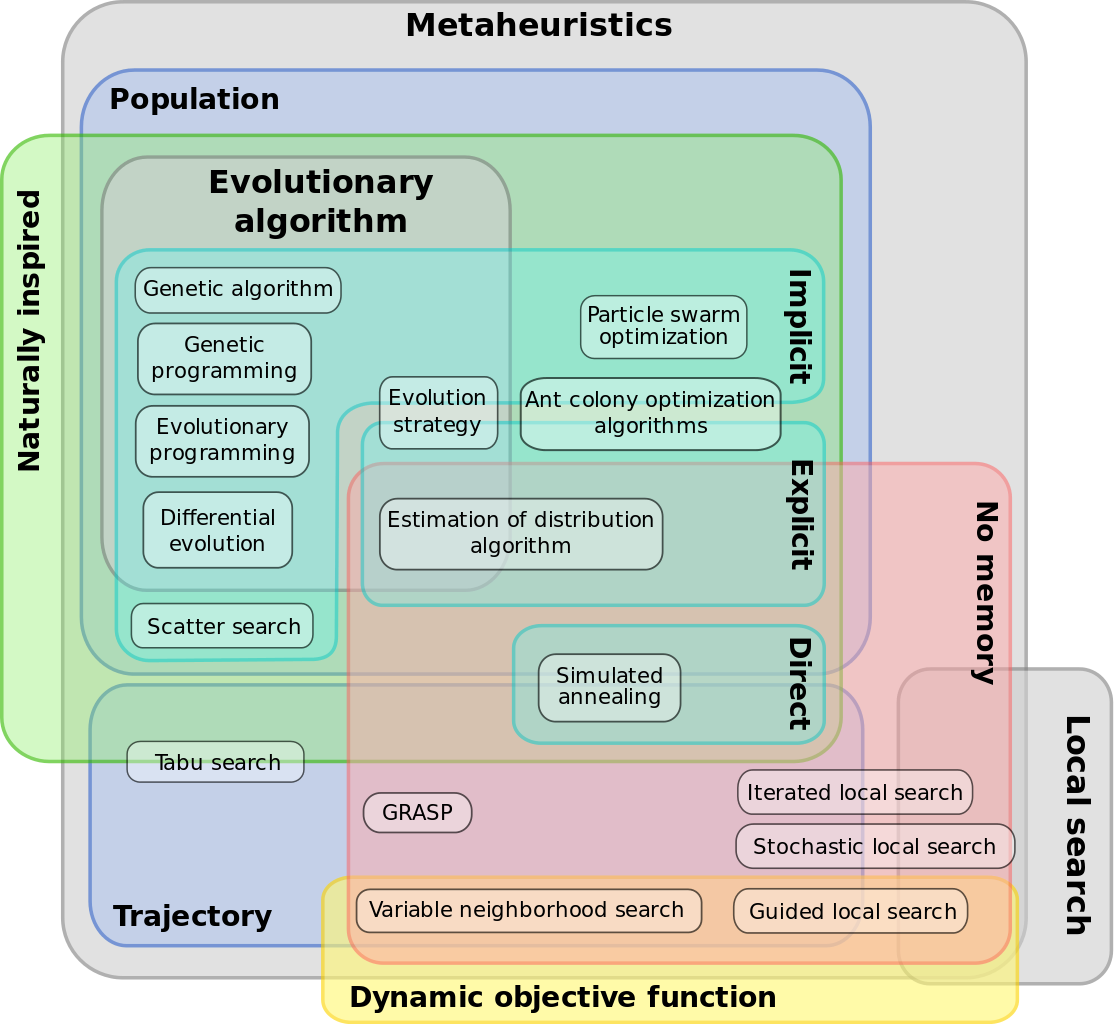
\includegraphics[width=0.7\textwidth]{graphics/Background/Metaheuristics_classification}
	\caption{Meta-heuristics Classification.}
	\label{BG: MH classification}
\end{figure}

As an example, the authors in~\cite{birattari2001classification} highlight the following classification facets:
\begin{itemize}
	\item The \textbf{walk-through search space method} could be either trajectory based or discontinuous. The first one corresponds to a closed walk on the neighborhood where such prominent examples as the \textit{iterated local search}~\cite{lourencco2003iterated} or the \textit{tabu search}~\cite{glover1989tabu} do exist. The second one allows large jumps in the search space, where the examples are such MHs as the \textit{variable neighborhood search}~\cite{hansen2003variable} or the \textit{simulated annealing}~\cite{kirkpatrick1983optimization}.
	
	\item The \textbf{number of concurrent solutions} could be either single or multiple. Such approaches as tabu search, simulated annealing or iterated local search are the examples of algorithms with a single concurrent solution. The evolutionary algorithms~\cite{eiben2015evolutionary}, the ant colony optimization~\cite{dorigo2007ant} or the particle swarm optimization~\cite{kennedy1995particle} are the instances of algorithms with multiple concurrent solutions (the population of solutions).
	
	\item From the \textbf{memory usage} perspective, we distinguish those approaches which do and do not utilize the memory. The tabu search explicitly uses memory in form of tabu lists to guide the search, but the simulated annealing is memory-less.
	
	\item The \textbf{neighborhood structure} could be either static or dynamic. Most local search algorithms, such as the simulated annealing and tabu search are based on the static neighborhood. The variable neighborhood search is an opposite case, where various structures of neighborhood are defined and interchanged while the algorithm solves the OP. 
\end{itemize}

There are many more classification facets, with are not in the scope of this thesis. \cref{BG: MH classification} illustrates the summarized classification including some characteristics and well-known meta-heuristic instances we did not mention~\cite{wiki_MH_classification}.


\subsubsection{Meta-Heuristics Examples}\label{BG: MH Examples}
At this point, let us briefly describe some of the most prominent and widely used meta-heuristics. It is motivated by the later usage of them as the LLH in hyper-heuristic, described in the \cref{impl: LLH}.

\paragraph{Evolutionary Algorithms (EAs).} 
They are directly inspired by the processes in nature, described in evolution theory. The common underlying idea in all of these methods is as follows: if we put a population of individuals (solutions) into an environment with limited resources (population size limit), a competition processes cause natural selection, where only the best individuals survive~\cite{eiben2015evolutionary}.

Tree basic actions are defined as operators of EAs: the \emph{recombination} operator selects the parent solutions, which later will be combined to produce the new ones (offspring); \emph{mutation} operator, when applied to solution, creates a new and very similar one. Applying both operators, algorithm creates a set of new solutions — the offspring, whose quality is then evaluated on TS. After that, the \textit{selection} operator is applied to all available solutions (parents and offspring) to keep the population size within the defined boundaries. This process is repeated, until some termination criteria is fulfilled. For instance, the maximal iterations counter reached, the number of TS evaluations exceeds, or the solution with required quality is found. The work-flow of EA depicted on the \cref{bg:pic:EAs}.

\begin{figure}
	\centering
	\includesvg{EA}
	\caption{Evolutionary Algorithms Workflow.}
	\label{bg:pic:EAs}
\end{figure}

The well-known examples of EAs include the \textit{genetic algorithm}~\cite{sastry2005genetic}, \textit{genetic/evolutionary programming}~\cite{koza1992evolution}, \textit{evolution strategies}~\cite{beyer2002evolution}, and many other algorithms.

\emph{Genetic Algorithm} (GA) is the first of all associated with the Evolutionary Algorithms. GA traditionally has a fixed workflow: given an initial population of $\mu$ usually randomly sampled individuals, the parent selection operator creates pairs of parents where the probability of each solution to become a parent depends on its objective value (fitness, or results). After that, the crossover operator is applied to every created pair with the probability $p_c$ and produces children. Then, newly created Solutions undergo the mutation operator with the independent probability $p_m$. The resulting offspring perform a tournament within the selection operator and $\mu$ survivals replace the current population~\cite{eiben2015popular}. Distinguishable characteristic of vanilla GA is the usage of following operators: bit-strings solution representation, one-point crossover recombination, bit-flip mutation and generational selection (only children survive).

\emph{Evolution Strategy} (ES), comparing to GA, are working in a vector space of the solution representation. However, they also use the population size of $\mu$ individuals and $\lambda$ offspring generated in each iteration. While the general workflow for all EAs remains the same, they mostly differ in underlying operators. In ES, the parent selection operator takes a whole population into consideration uniformly, the recombination scheme could involve more than two parents to create one child. To construct a child, the recombination operator joins parents alleles in two possible ways: (1) with uniform probability for each parent (discrete recombination), or (2) averaging the weights of alleles by parent solution quality (intermediate recombination). There are two selection schemes, used in such algorithms: $(\mu,\lambda)$ — discard all parents and selecting only among offspring highly enriching the exploration, and $(\mu+\lambda)$ — include also the predecessor solutions into selection, which is often called the \textit{elitist selection}~\cite{eiben2015popular}. In many cases, the ES utilizes a very useful feature of \emph{self-adaptation}: changing the mutation step sizes in a runtime, which we will discuss in dedicated to Parameter Control \cref{bg: parameter control}.

\paragraph{Simulated Annealing (SA).} This is the other type of meta-heuristics, inspired by the technique used in metallurgy to obtain `well-ordered' solid state of metal~\cite{van1987simulated}. An annealing technique imposes a globally minimal internal energy state and avoids locally minimal semi-stable structures. 

The SA treats the search process as the metal with a high temperature at the beginning and lowering it to minimum while approaching the end. %SA algorithm handles the optimization objective as annealing threat the material energy. 
It starts with an initial solution $S$ creation (randomly or using some other heuristic) and temperature parameter $T$ initialization. At each iteration, a new solution candidate is sampled within a neighborhood of current solution: $S^* \leftarrow N(S)$. The newly sampled solution replaces the older one, if (1) optimization objective $f(S^*)$ dominates over $f(S)$ or (2) with a probability that depends on quality loose and current value of $T$, see \cref{bg: SA acceptance criteria}.

\begin{equation}
p(T, f(S^*), f(S)) = \exp(-\frac{|f(S^*) - f(S)|}{T})
\label{bg: SA acceptance criteria}
\end{equation}

At each iteration the temperature parameter $T$ value is decreased following some type of annealing schedule, which is also called as \textit{cooling rate}~\cite{boussaid2013survey}. The weak side here is that the quality of each annealing schedule is the problem dependent and cannot be determined beforehand. Nevertheless, the SA algorithms with parameter control do exist and address this problem changing the cooling rate or temperature parameter $T$ during the search process. Later, we will shortly review these techniques in the \cref{bg: parameter control: SA}.


\subsection{Hybrid-Heuristics}
The hybridization of different systems often provides a positive effect — taking the advantages of one system and merging them with characteristics of the other, getting the best from both systems. The same idea is applicable in case of meta-heuristics. Imagine you have two algorithms, one is biased towards exploration, the other — towards exploitation. Applying them separately, the expecting results in most cases may be far away from the optimal as the outcome of disrupted diversification-intensification balance. But, when merging them into, for example, repeated stages of hybrid heuristic, one will obtain the advantages of both escaping a local optima and finding a good quality result. 

Most of available hybridization are created with the help of this idea of two heuristics staging combination, one of which is suited for the exploration and other is better for the exploitation.

The methods to construct the hybrids are mostly defined by the underlying heuristics therefore, to the best of our knowledge they could not be generalized and classified in an appropriate way. The only one commonly shared characteristic is the usage of \textit{staging approach}, where the output of one algorithm is used as initial state of the other. 

As for the simple heuristics, we introduce some examples of performed hybridization in order to provide the reader a better understanding of useful for the hybridization parts of algorithms and influence of the aforementioned balance on the search process.

\subsubsection{Hybrid-Heuristics Examples}
\paragraph{Guided Local Search and Fast Local Search.}
The main focus of GLS in this case, lies on the search space exploration and the guidance of process using incubated information. To some extent, the GLS approach is closely related to the frequency-based memory usage in tabu search. During the runtime, GLS modifies the problem cost function to include penalties and passes this modified cost function to the local search procedure. These penalties form a memory that characterizes a local optimum and guide the process out of it. The more time algorithm spends in local optimum — the higher penalties. A local search procedure is carried out by the FLS algorithm, where the main advantage is a quick neighborhood traversal. It is done by braking it up into a number of small sub-neighborhoods. Afterwards, by performing the depth first search over these sub-neighborhoods, it ignores those, without an improving moves. At some point of the time FLS reaches the local optimum and passes back the control in GLS to update the penalties and repeat the iteration~\cite{tsang1997fast}.

\paragraph{Direct Global and Local Search.}
This hybridization consists of two stages: the stochastic global coarse pre-optimization and the deterministic local fine-optimization. In the first stage, authors apply one of the two mentioned earlier meta-heuristics: the Genetic Algorithm or the Simulated Annealing. The transition from global to local search happens after reaching the predefined conditions. For instance, when the number of TS evaluations exceeds a boundary, or when no distinguishable improvement made in the last few iterations. Then, the pattern search algorithm~\cite{hooke1961direct} also known as the direct, derivative-free, or black-box search performs the fine-optimization. The hybrid-heuristic terminates when the pattern search converges to local optima~\cite{syrjakow1999efficient}.

\paragraph{Simulated Annealing and Local Search.}
After the brief explanation of previous two hybrids, an observant reader hopefully guesses, what is happening in this hybridization.
The authors in their work~\cite{martin1996combining} called this method the `Chained Local Optimization'. Thus, it is a yet another representative of staged hybridization.
Iteration starts with the current solution perturbation, called \emph{kick} in~\cite{martin1996combining}, referring a dramatic change of current position within the search space. Afterwards, the hill climbing algorithm is applied to intensify the obtained solution. When reached the local optimum, hill climber passes the control flow back to the simulated annealing for acceptance criteria evaluation, which finishes the iteration.

\paragraph{EMILI.}
Easily Modifiable Iterated Local search Implementation (EMILI) is a framework system for the automatic generation of new hybrid stochastic local search algorithms~\cite{pagnozzi2019automatic}. EMILI is a solver for permutation flow-shop problems (PFSP), also known as flow shop scheduling problems~\cite{reza2005flowshop}. In PFSP the search of an optimal sequence of steps to create products within a workshop is performed.
In this framework, the authors have implemented both generic algorithmic- and problem-specific building blocks. They also have defined grammar-based rules for those blocks composition and used an automatic parameter tuning tool IRACE~\cite{lopez2016irace} to find the high performing algorithm configurations. The workflow of EMILI could be split in three steps: (1) adaptation of the grammar rules to specific PFSP objective representations (make-span, sum completion times and total tardiness), (2) generation of all possible hybrid heuristics for each PFSP representation and (3) execution of IRACE to select the best performing hybrid for each problem. 

From our perspective, the described approach of automatic algorithm generation is an example of construction hyper-heuristics, which we describe in the upcoming \cref{bg: hh}. However, we are not authorized to change the system class (from hybrid- to hyper-heuristic) defined by the EMILI authors.

\todoy{or we can move it into the hyper-heuristics, stating that we think, it should be there?}

\todoy{continue proofreading here}

\subsection{No Free Lunch Theorem}
A nature question could arise ``If we have all this fancy and well-performing heuristics, why should we put an effort in developing new algorithms, instead of using the existing?'' And the answer to this question is quite simple — the perfect algorithm suited for all OP does not exist and can not exist. 
The empirical research has shown that some meta-heuristics perform better with some types of problems, but poorly with others. In addition to that, for different instances of the same problem type, the same algorithm could result in unexpected performance metrics. Moreover, even in different stages of same problem solving process the dominance of one heuristic over another could change. 

All search algorithms perform exactly the same, when the results are averaged over all possible Optimization Problems. If an algorithm is gaining the performance in one problems class, it loses in another class. This is a consequence of so-called \textbf{No Free Lunch Theorem for Optimization} (NFLT)~\cite{wolpert1997no}.

In fact, one could not predict, how exactly will behave one or another algorithm with problem in hand. A possible and the most obvious way is to probe one algorithm and compare its performance to another one during problem solving process. In this case simple heuristics and meta-heuristics are out of competition, since once you solved the Optimization Problem you probably wouldn't optimize a second time.
Here come \textbf{Hyper-Heuristics} to intelligently pick heuristics that is suitable to problem in hand. We will proceed with their description and how they deal with the NFLT consequences in following section.


\subsection{Hyper-Heuristics}\label{bg: hh}
A lot of state-of-the-art heuristics and meta-heuristics are developed in a complex and very domain-dependent way, which causes problems in an algorithm implementation reuse. It motivated research community to raise the level of generality at which the optimization systems can operate and still provide good quality Solutions for various Optimization Problems. 

The term \textbf{Hyper-Heuristic} (HH) was defined to describe an approach of using some \textit{High-Level-Heuristics} (HLH) to select over other \textit{Low-Level-Heuristics} (LLH) and apply them to solve the \textit{class of Optimization Problems} rather than particular instance. Indeed, scientists report that the combination of different HLH produces better results than if hey were applied separately~\cite{drake2019recent} — note previously discussed hybrid-heuristics.
This behavior can be explained by the nature of search process and how it evolves in time. When you apply a heuristic, it sooner or later converge to some extreme point, hopefully global optimum. But it is `blind' to other, not visited regions in the Search Space. Changing the trajectory of investigation by (1) drastically varying the Neighborhood, (2) changing the strategy of Neighborhood exploration and exploitation could (1) bring you to those previously unreachable zones (2) in more rapid ways. However, usually it is hard to predict how one LLH will behave in every stage of the search process in comparison to another. In Hyper-Heuristics, this job was encapsulated into the HLH and performed automatically. 

In~\cite{moriarty1999evolutionary} authors made infer that Hyper-Heuristics can be viewed as a form of Reinforcement Learning, which is a logical conclusion especially if we rephrase it to \textit{Hyper-Heuristics utilize Reinforcement Learning methodologies}.

\begin{figure}
	\centering
	\includesvg{HH}
	\caption[Hyper-Heuristics]{Hyper-Heuristics.}
	\label{bg:pic:HH}
\end{figure}

The new concept which implicitly was used in Meta-Heuristics, but explicitly pointed out in Hyper-Heuristics is the \textbf{Domain Barrier} (\cref{bg:pic:HH}\footnote{Icons from \href{thenounproject.com/}{thenounproject.com}}).
As we told previously, HH do not tackle the OP directly, but use LLH instead. This means, that usually HH are minimally aware of the domain details, such as what are data types, relationships, etc. within a domain. This information rather encapsulated in LLHs, thus HHs could be used to broader range of Optimization Problems.

With this idea, many researchers started to create not only Hyper-Heuristics to tackle a concrete optimization problem class, but also frameworks with building blocks for their creation.


\subsubsection{Classification}
Although, the research in Hyper-Heuristics field is actively ongoing, many algorithm instances were already created and some trials to organize approaches were conducted in~\cite{ryser2014review,drake2019recent,burke2019classification}.

Researchers in their surveys classify HHs by different characteristics, some of which overlap, but it also happens that important (from our perspective) features were not highlighted in all works. 

In this section we present the union of those important Hyper-Heuristics classification facets to better justify the goal of this thesis.

We begin with the two broadest classes, which differentiate HH \textbf{routine}, also called as \textbf{nature of High-Level-Heuristic Search Space}~\cite{burke2013hyper,burke2019classification,drake2019recent}.
The first class are Hyper-Heuristics to \textit{select} Low-Level-Heuristic, in other words \textit{Selection Hyper-Heuristic}. All our previous references to Hyper-Heuristics were made this concrete type. These algorithms operate in the Search Space, defined by complete and rather simple Low-Level-Heuristics that solve Optimization Problem. The task of HLH here is to pick the best suited LLH (or sequence of LLHs) based on available prior knowledge and apply it to the OP underway. Note, that staging Hybrid-Heuristics could be viewed as Solutions of Selection HHs.
Hyper-Heuristics of the second class seek to \textit{construct} LLH following some predefined receipt and using the atomic components of other heuristics as Lego bricks. The other commonly used name here is \textit{Construction Hyper-Heuristics}. These approaches often lead to creation of new and unforeseen heuristics that are expected to reveal good performance while solving the problem in hand.

Next, the distinction in \textbf{nature of Low-Level-Heuristics Search Space} arises. 
In other words: ``How does the LLH derive Solutions for the OP?'' Authors in~\cite{burke2013hyper,burke2019classification,drake2019recent} distinguished \textit{construction} LLHs where Solution creation happens each time from scratch and \textit{perturbation} LLHs where new Solutions created from parts of already existing ones.

The other broadly used characteristic is the \textbf{memory usage method}. 
From this perspective we distinguish Hyper-Heuristics in which the learning happens \textit{on-line}, \textit{off-line} or learning mechanisms are \textit{not present} at all~\cite{ryser2014review,burke2019classification}.
\begin{itemize}
	\item In \textbf{on-line} case, the HH derives an information, used to select among LLH, while those LLH are solving the problem.

	\item In \textbf{off-line} case, the learning happens before solving concrete Optimization Problem. Here one should first train an HH solving other homogeneous problem instances by underlying LLHs (off-line learning phase). After that, the HLH will be able to choose among LLHs, thus be applicable to problem in hand (on-line use phase). Note, that this approach also requires creation of meta-features extraction mechanism and its application to every Optimization Problem.

	\item There exist also \textbf{mixed} cases, where learning happens first in off-line and later also in on-line phase. Definitely it is a promising (in terms of results quality) research direction, despite it high complexity.
	
	\item In the last case \textbf{no learning} mechanisms present, therefore HLH here performs some sort of Random Search over LLH Search Space. At first sight, it may look like weak approach, but looking onto Variable Neighborhood Search Meta-Heuristic we would doubt it.
\end{itemize}


%Yet another faced of Hyper-Heuristics classification is the way of assigning \textit{hyper-parameters} (here we use parameters and hyper-parameter concepts interchangeably) for LLHs, or their components~\cite{drake2019recent}. We analyzed surveys and find out that some researchers do not explicitly differentiate approches with respect to nature of parameter settings~\cite{ryser2014review,burke2013hyper,burke2019classification}, while other do~\cite{drake2019recent}:
%\begin{itemize}
%	\item In \textbf{static} assignment, the underlying heuristics use provided beforehand (usually default) hyper-parameters and do not change them while solving the problem in hand.

%	\item The \textbf{dynamic} case uses some kind of rule for parameters changing, specified in advance.

%	\item There exist also an \textbf{adaptive} approach, in which HH assigns the parameters for LLH as the response to the learning process. In some sort, it is similar to the parameter control techniques used in Meta-heuristics.
	
%	\item And finally, a \textbf{self-adaptive} approach where underlying LLHs comprise \textit{parameter control} techniques, thus search for the best solution for OP and own parameter settings simultaneously.
%\end{itemize}


For more detailed analysis, description, other classification facets and respective Hyper-Heuristic examples we encourage reader to look into resent classification and surveying researches~\cite{burke2003hyper,ryser2014review,drake2019recent,burke2019classification}.

\subsubsection{Hyper-Heuristics Instance Examples}\label{bg: hh examples}
\paragraph{Hyper-Heuristic for Integration and Test Order Problem~\cite{guizzo2015hyper}.} \textit{HITO} is an example of generational HH. LLHs in this case are presented as a composition of basic EAs operators — crossover and mutation forming multi objective evolutionary algorithms (MOEA). HH selects those components from $jMetal$ framework~\cite{durillo2011jmetal} using interchangeably Choice Function (in form of weighted linear equation) and Multi Armed Bandit based Heuristic to balance exploitation of good components and exploration of new promising ones.


\paragraph{Markov Chain Hyper-Heuristic~\cite{mcclymont2011markov}.} \textit{MCHH} is an on-line selective Hyper-Heuristic for multi-objective continuous problems. It utilizes reinforcement learning techniques and Markov Chain approximations to provide adaptive heuristic selection method. While solving the OP, \textit{MCHH} updates prior knowledge about the probability of producing Pareto dominating Solutions by each underlying LLH using Markov Chains, thus guiding an LLH selection process. Applying on-line reinforcement learning techniques, this HH adapts transition of weights in the Markov Chains constructed from all available LLHs, thus updating prior knowledge for LLH selection.


\subsubsection{Hyper-Heuristics Frameworks Examples}\label{bg: hh fw examples}
\paragraph{Hyper-Heuristics Flexible Framework~\cite{ochoa2012hyflex}.} \textit{HyFlex} is a software skeleton, built specifically to help other researchers creating Hyper-Heuristics. It provides the implementation of components for 6 problem domains (Boolean Satisfiability, Bin Packing, Personnel Scheduling, Permutation Flow Shop, Traveling Salesman and Vehicle Routing problems), such as problem and solution descriptions, evaluation functions and adaptations for set of Low-Level-Heuristics. The set benchmarks and comparison techniques to other built HHs on top of \textit{HyFlex} are included to framework as well. 

The intent of \textit{HyFlex} creators was to provide Low-Level features that enable others to focus directly on High-Level-Heuristics implementation without need to challenge other minor needs. It also brings a clear comparison among created HLH performance, since the other parts are mostly common. From the classification perspective, all derivatives from the \textit{HyFlex} framework are Selection Hyper-Heuristics, however they utilize different learning approaches. Algorithms, built on top of \textit{HyFlex} framework could be found in many reviews~\cite{misir2012intelligent,ryser2014review,drake2019recent} or on the CHeSC 2011 challenge website\footnote{\href{http://www.asap.cs.nott.ac.uk/external/chesc2011/}{Cross Domain Heuristic Search Challenge website: asap.cs.nott.ac.uk/external/chesc2011/}} (dedicated to choosing the best HH built on top of \textit{HyFlex}).

Along with \textit{HyFlex}, a number of hyper-heuristic-dedicated frameworks is growing, some of them are under active development while others are abandoned:
\begin{itemize}
	\item \textbf{Hyperion}~\cite{swan2011hyperion} is a construction hyper-heuristic framework aiming to extract information from the OP search domain for identification of promising components in form of object-oriented analysis.
	
	\item \textbf{hMod}~\cite{urra2013hMod} framework allows not only to rapidly prototype an algorithm using provided components, but also to construct those components using predefined abstractions (such as $IterativeHeuristic$). In current development stage, developers of \textit{hMod} are focusing on creation of development mechanisms rather than providing a set pre-built heuristics. 
	
	\item \textbf{EvoHyp}~\cite{pillay2017evohyp} framework focuses on hyper-heuristics created from evolutionary algorithms and their components. Here authors enable framework users to construct both selection and generation HHs for both construction and perturbation LLHs types.
\end{itemize}


\subsection{Conclusion on Heuristic Solvers}
To conclude our review on Heuristic approaches for solving Optimization Problems, we shortly remind you pros and cons of each heuristic level.

On the basis remain Simple Heuristics with all their domain-specific knowledge usage and particular tricks for solving problems. Usually, they are created to tackle a concrete problem instance in hand applying simple algorithmic approach. The simplicity of application and usually fast runtime paid back by medium results quality.

On the next level inhabit Meta-Heuristics. They could be compared with more sophisticated Solutions hunters which could not only charge directly, but also take a step back when stuck in a dead end. This additional skill enables them to survive in new and complex environments (Optimization Problems), however some adaptations to understand a concrete problem and parameter tuning for better performance still should be performed.

Among with MHs exit Hybrid-Heuristics. There is nothing special here, they just took some survival abilities from several Meta-Heuristics hoping to outperform and still requiring adaptation and tuning. In some cases this hybridization provides it advantage, but as the time shows, they did not force out MHs. Those we can conclude that the provided balance between development effort and exposed results quality not always assure users to use them.

Finally, the chosen ones that lead the others, Hyper-Heuristics are on the upper generality level. 
Operating by the other Heuristics, HHs analyze how good former are and make use of this knowledge by solving the concrete problem using those best suited Heuristics. Imposing such great abilities, Hyper-Heuristics tackle not only the concrete optimization problem, but entire class of problems.


\section{Setting Algorithm Parameters}\label{bg: section Parameters Setting}
The most of existing learning algorithms expose some parameter set, needed to be assigned before using this algorithm. Modifying these parameters, one could change the system behavior and possible result quality.

When we are talking about the problem of settings the best parameters, following terms should be refined explicitly:
\begin{enumerate}
	\item \textbf{Target System (TS)} is the subject which parameters are undergoing changes. Simply, it could be a heuristic, machine learning algorithm or other system.
	\item \textbf{Parameter} is one of exposed by TS setting hooks. It should be described in terms of its type and possible values.
	\item \textbf{Configuration} is the unique combination of parameter values, sufficient to run TS.
	\item \textbf{Search Space} is the set of all possible Configurations for defined Parameters.
\end{enumerate}

In this thesis we use notions of \textit{Parameter} and \textit{Hyper-Parameter} (HP) interchangeably, since the approaches discussed in this section are generally applicable also in Machine Learning cases. For instance, consider Neuron Network (NN). Hyper-parameters in this case will specify the structure (number of hidden layers, units, etc.) and learning process (learning rate, regularization parameters values, etc.) of network and changing them dramatically affect performance and results.

One frequent incumbent of Optimization Problems is \textbf{Parameter Settings Problem} (PSP) — searching of hyper-parameter values that optimize some characteristic of TS. When talking about NN example, PSP could be defined as task of maximization network accuracy in given dataset (Single Objective PSP). Taking into account a number of TS characteristics simultaneously, such as training time and prediction accuracy PSP transforms into Multi-Objective PSP.

The same applies to heuristics: proper assignment of hyper-parameters has a great impact on exploration-exploitation balance and thus on overall algorithm performance.

Up until now there were formalized many approaches for solving task of settings hyper-parameters. 
One of the simplest and error-prone ways is just trusting your (or someones else) intuition and using those parameters that seems more or less logical for particular system under the problem instance. People quickly abandoned it in favor of automatic approaches, fortunately novel computational capacities easily provide a possibility for it. These automatic methods later could be split onto \textit{off-line or parameter tuning} and \textit{on-line or parameter control} techniques.

\todoy{interesting visualization scheme on page 366 $https://link.springer.com/chapter/10.1007/978-3-642-29178-4_37$}

\subsection{Parameter Tuning}\label{bg: parameter tuning}
Roughly speaking, the off-line approach is a process of traversing the search space of hyper-parameters and evaluating TS with these parameters on some set of toy problems. After finishing this process, the best found HPs are later used to solve new, unforeseen problem instance.

In this part of thesis we briefly outline existing automated approaches for parameter tuning illustrating them on the \cref{bg: fig:automated parameter tuning approaches}\footnote{Original graphics are taken from~\cite{koch2017automated}}. In this example, the TS exposes two parameters: $X_1$ and $X_2$. Each graphic shows dependencies between $X_1$ (horizontal axis) and $X_2$ (vertical axis) values and the subject of optimization along those axes (here depicted the maximization case). The best found configuration by each approach is highlighted in pink.

\begin{figure}
	\centering
	\begin{subfigure}[b]{0.25\linewidth}
		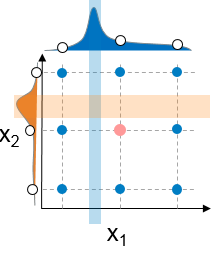
\includegraphics[width=\linewidth]{graphics/Background/hyperparameter-grid-search.png}
		\caption{Grid.}
		\label{bg: fig:automated parameter tuning approaches: grid}
	\end{subfigure}
	\begin{subfigure}[b]{0.25\linewidth}
		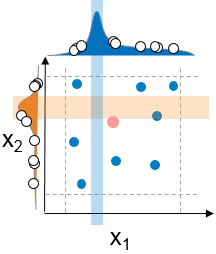
\includegraphics[width=\linewidth]{graphics/Background/hyperparameter-random-search.png}
		\caption{Random.}
		\label{bg: fig:automated parameter tuning approaches: random}
	\end{subfigure}
	\begin{subfigure}[b]{0.25\linewidth}
		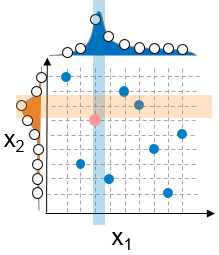
\includegraphics[width=\linewidth]{graphics/Background/hyperparameter-learning-search.png}
		\caption{Learning.}
		\label{bg: fig:automated parameter tuning approaches: learning}
	\end{subfigure}
	\caption{Automated Parameter Tuning Approaches.}
	\label{bg: fig:automated parameter tuning approaches}
\end{figure}

\paragraph{Grid Search Parameter Tuning.} It is a rather simple approach for searching parameters. Here the original search problem is relaxed and later solved by brute-force algorithm. The set of all possible configurations (parameter sets) for relaxed problem is derived by specifying a finite number of possible values for each hyper-parameter under consideration. After evaluating all configurations on TS, the best found solution is reported. As you can see, this approach could skip promising parts of search space (\cref{bg: fig:automated parameter tuning approaches: grid}).

\paragraph{Random Search Parameter Tuning.} This methodology relies on random (often uniform) sampling of hyper-parameters and their evaluation on each iteration. At first sight, it might look unreliable to chaotically traverse the search space. But empirical studies show that with growing number of evaluations this technique starts to outperform grid search~\cite{bergstra2012random}: compare the best configurations (highlighted in pink) found by grid (\cref{bg: fig:automated parameter tuning approaches: grid}) and random search (\cref{bg: fig:automated parameter tuning approaches: random}) techniques.

\paragraph{Model Based Search Parameter Tuning.} In the most cases, the dependencies between tuned parameter values and optimization objective do exist and can be utilized for hyper-parameter tuning. By predicting which parameter combinations lead to better results, model-based tuning could make precise guesses. As it showed on the \cref{bg: fig:automated parameter tuning approaches: learning}, at the beginning, this approach behaves as random search, but after accumulating enough information, learning algorithm starts making more precise guesses, which in contrast to previously described model-free approaches is desirable and more robust.

Naturally, this optimization problem could be tackled by almost every discussed here approach, however taking into account the facts that (1) TS here in most cases is a \textit{black-box} we eliminate exact and approximate solvers, (2) the evaluation cost is huge, thus it is not desirable to apply any of described above heuristics directly.

With this idea in mind, researchers started to (1) create  Bayesian optimization algorithms that traverse the search space more efficiently and (2) build models that could recreate the dependencies between parameters and objective values, a so-called \textit{surrogate models}. While the former direction is nothing else but an enhancement to already existing optimization techniques, the later one is crucial for problems where objective is expensive to evaluate.
The later is some sort of enhancement used in combination with former enabling you to simulate evaluation of real system instead of expensive direct evaluations. Still, it is a common approach to combine previously reviewed search space traversal techniques, such as evolutionary algorithms, simulated annealing, tabu search with surrogate models for optimization.


\subsection{Systems for Model-Based Parameter Tuning}\label{bg: parameter tuning expamples}
The parameter tuning is an obligatory task when the maximum system performance is a mast-have requirement and should be performed at the design time.
Novel tuning approaches are usually built in form of frameworks with exposed hooks for attaching the system under estimation.

Since, the target system evaluations here supposed to be extremely costly, thus parameter tuning frameworks are trying to utilize every single bit of information from evaluations by building surrogate models and using Bayesian optimization approaches is obligatory.

In this section we review some among existing open-source parameter tuning systems from following perspectives:
\begin{itemize}
	\item \textbf{Conditional parameters support} is (1) a provided for user and (2) handled by tuning system ability to describe conditional dependencies between hyper-parameters. As an example, imagine \textit{crossover type} parameter of Genetic Algorithm that can take only some specific values: \textit{Partially Mapped Crossover ($PMX$)}, \textit{Cycle Crossover ($CX$)}, etc. Binding concrete crossover type, one will be required provide parameters for this crossover type, but eliminate respective parameters for other crossover types. This type of dependency could be described in form of parent-child relationship, however other types of dependencies also exists.
	
	\item \textbf{Parameter types support} is one of the basic usable tuning systems requirements. More concretely, Target System parameters could be not only numerical (integer or fractional), but also categorical in form of strings, boolean values, etc. Considering categorical data types, they could be either \textit{nominal} (depict only possible atomic values) or \textit{ordinal} (implies also value comparison, but no distance notion). For instance lets again analyze parameters of Genetic Algorithm: population size — numerical integer in range $[1...\inf)$, mutation probability — numerical fractional $[0...1]$, crossover type — categorical nominal ${PMX, CX}$. Indeed, we could treat population size as a set of finite values ${10, 100, 1000}$ — categorical ordinal parameter type.
	
	\item \textbf{Extensibility} is crucial when someone would like to try a new promising and intriguing learning algorithm for guiding a search, that was not available in parameter tuning system yet. Practically, one may need not only new learning algorithm, but some other features like non-trivial stopping criterion, tools for handling stochastic behaviors, or different strategies for random sampling (which are utilized while tuning system is learning before making a prediction).
	
	\item \textbf{Parallel Evaluations} required for utilizing available computing resources that could scale horizontally, thus providing simultaneous evaluation of multiple Configurations which speeds-up the learning process.
\end{itemize}

Among reviewed systems we could distinguish ones that were created directly to face the parameter tuning problem and the others that are more generic optimizers but still applicable in parameter tuning cases.
A concrete optimizer will be usable for searching the parameters, if it exposes several features. First, it must consider optimization function evaluation to be expensive and tackle this problem explicitly. For instance, using surrogate models or the other TS approximations. Next, potential tuner should be able to tackle dependencies and conditions among parameters.

\subsubsection{SMACv3~\cite{hutter2011sequential}}\label{bg: smac}
Sequential Model-based Algorithm Configuration (SMAC~\footnote{SMACv3 GitHub repository~\url{https://github.com/automl/SMAC3/}}) is a system for parameters tuning, developed by the AutoML research group (here we review a $3^rd$ version of SMAC). 

In their research, scientists generalized the process of parameter tuning under the  \emph{Sequential Model-Based Optimization} (SMBO) term as the iterations between (1) fitting models and (2) using them to choice next configurations for evaluation. 
We found this term naturally formalizes the most of existing (to the best of our knowledge) parameter tuning approaches and may be used as a distinguishing characteristic of optimization algorithms (since they naturally could be applied not only to parameter tuning problems).

SMACv3 is an extension introducing the learning models and sampling mechanisms to previously existing random on-line aggressive racing (ROAR) algorithm. Authors showed the machine learning in general and regression models in particular (playing the role of surrogate models) are applicable not only for parameter tuning, but also for optimizing any expensive black-box functions in general. 

The development of this system was motivated to tackle the existing limitations of all published SMBO approaches namely, expanding an applicability not only to numerical, but also to categorical parameters and optimizing the target algorithm performance not only on single, but on number of problem instances (benchmark set), reducing the variance influence.

A routine in SMAC could be viewed as an iterated application tree steps: (1) building a learning model, (2) using it for making choices which configurations to investigate next and (3) actual evaluation of the sampled configurations.

The evaluation (3) here carried out by the original ROAR mechanism, where the evaluation of each new candidate solution continues until enough data (from benchmark set of problem instances) obtained to either replace the current solution or reject the candidate. In a contrary to model-less ROAR, SMAC at step (1) builds the regression random forest — an instance of machine learning algorithm~\cite{breiman2001random}. The usage of the regression decision trees is motivated by the fact that they fit well to categorical data and complex dependencies in general. Later, at step (2) the iterative local search (ILS) heuristic applies in combination with \emph{Expected Improvement} (EI) evaluation (form of the Bayesian optimization)~\cite{shahriari2015taking}. ILS starts at the best previously found configuration and traverses its neighborhood distinguishing between configurations using EI and regression model built at step (1). EI is large for those configurations, which has low predicted cost and for those, with high uncertainty in results therefore, naturally providing the exploration-exploitation balance~\cite{jones1998efficient}.


\subsubsection{IRACE}\label{bg: irace}
IRACE~\footnote{IRACE GitHub repository~\url{https://github.com/MLopez-Ibanez/irace}} is hyper-parameter tuning package~\cite{lopez2016irace} as the implementation of Iterated Racing Algorithm~\cite{birattari2010f}.

The underlying methodology is somehow similar to one implemented in SMACv3 and comprise three main steps: (1) sampling new configurations using a prior knowledge, (2) empirically finding the best ones among sampled using the racing algorithm and (3) updating the prior knowledge to bias future samples in towards better configurations. The prior knowledge here is represented as the probability distributions of values for each parameter independently (truncated normal and discrete distributions for numeric and categorical hyper-parameters respectively). During update step (3), the probability distributions are build using the best found in (2) step configurations therefore, increasing the sampling possibilities for the promising values.

Iterated racing step (2) here is a process of running the target system using sampled configuration on a set of problem instances. After solving each instance, the statistically worse-performing configurations are rejected and racing proceeds with remaining ones. This process continues until reaching the required number of survivals, or after solving a requiring amount of problem instances (in this case all remaining configurations are considered to be good). 

IRACE supports various data types, such as numerical or categorical and the possibility of conditions description as well. While the problem of data types solved by different underlying distributions, the conditional relationships are handled by the dependency graphs. During sampling (1), firstly the non-conditional parameters are sampled and only afterwards, if respective conditions are satisfied, the dependent parameters are sampled.


\subsubsection{HpBandSter}\label{bg: bohb}
A distributed Hyperband implementation on Steroids (HpBandSter~\footnote{HpBandSter GitHub repository: \url{https://github.com/automl/HpBandSter}}) is the realization of BOHB algorithm~\cite{falkner2018bohb} in the software framework.
While SMAC outperforms and partially reuses the decisions made in ParamILS, BOHB (Bayesian Optimization combined with HyperBand) is the parameter tuning tool that outperforms SMAC and was created by the same AutoML research group.

As it stated in name, the SMBO routines in this framework are carried out with mainly two algorithms: (1) learning and configurations sampling done by the Tree Parzen Estimator (TPE, Bayesian Optimization technique), while (2) evaluation of sampled configurations and their comparison are carried out by the Hyperband (HB) algorithm.

The TPE usage instead of na\"ive Gaussian Processes-based (GP BO) Bayesian Optimization + Expected Improvement evaluation was motivated by a better dimensional scaling abilities and internal support of both numerical and categorical data types. However, some minor transformations are still required.
Unlike vanilla BO, where the optimization is done by modeling the result distributions given the configuration parameters, TPE builds two parameters distributions. It splits the configurations into two sets according to their `goodness'. During the sampling, it proposes those parameters, which have high probability to be in the `good' distribution and simultaneously low probability to be in the `bad' one. For more detailed explanation we refer to TPE description given in~\cite{bergstra2011algorithms}.

The central part of BOHB, namely the HyperBand is a promising bandit-based strategy for hyper-parameter optimization~\cite{li2017hyperband} in which the \emph{budget} for parameter tuning is defined beforehand and divided between iterations. The role of budget could play any control parameter that denotes the accuracy of configuration evaluation by TS, where estimation with the maximum budget gives you the most precise configuration evaluation, while the minimum amount of budget results in the least accurate approximation of configuration evaluation result.
The running examples of budget could be a number of iterations in iterative algorithm, a number of epochs to train the neuron network, or a number of problem instances from benchmark set to evaluate. As the result, requirements arise for TS to expose and support budget usage as expected in BOHB.

At each iteration, HB samples uniformly at random a number of configurations. The authors introduced an \emph{intensification} mechanism according to which, a number of per-iteration sampled configurations decreases for the later iterations, while the amount of budget given for iteration remains the same. As an outcome, first iterations of HB are full of coarse-grain evaluated configurations, while the later iterations produce a higher number of more precise measurements. Each iteration of HB is split to the number of \emph{Successful Halving} (SH) procedure executions which drop poorly performing configurations (usually $\sfrac{2}{3}$) at each execution. As one could expect, since the number of measured configurations in subsequent iterations decreases, the amount of SHs execution drops too therefore, the remaining configurations are evaluated more precisely.

The binding of HyperBand and Bayesian Tree Parzen Estimator is made in several places. Firstly, the learning models are updated each time, when new results are available for every budget value. Next, at each HB iteration instead of random sampling, the TPE model is used to pick next configurations. Note that \textit{BOHB} uses only those models, which built on configurations obtained for the largest budget. This decision results in more precise surrogate models (parameter distributions) and therefore, better predictions in the later stages of parameter tuning process.


\subsubsection{BRISEv2}\label{bg: brise}
The great part of software potential lays not only in its ability to tackle a problem in hand, but also on the general usability and adaptivity to unforeseen tasks.
Here we review a $2^{nd}$ version of BRISE\footnote{BRISEv2 GitHub repository: \url{https://github.com/dpukhkaiev/BRISE2/releases/tag/v2.3.0}}~\cite{brise2spl}, since the very early BRISE versions (major version 1~\cite{brise1monolite}) were more monolithic and hard to apply for parameter tuning problem in hand.

While designing this system, authors were focused not solely on learning mechanisms for parameter prediction, but on the overall system modularity as well.
Being a software product line (SPL), BRISE was designed as a set of interacting components (nodes), each acting according to its own specific role. 
The system could be viewed from two perspectives. One is a birds eye view on all available nodes with their roles and the other is a fine-grained description of~\textit{main-node} concretely.

Before reviewing each perspective, it is worth to justify the central terms used in system. Note, that some of them are pretty the same as we defined above, but here most of them also were implemented in form of classes.
\begin{enumerate}
	\item \emph{Experiment} encapsulates the information about a concrete run of BRISE. For instance, within a parameter tuning session it carries such information as BRISE experiment description (a specification of parameter tuning procedure in JSON format), all evaluated during session configurations with their results.

	\item \emph{Configuration} is a combination of input parameter values for target system, or algorithm under tuning. It could be run several times to obtain a statistical data therefore, contain number of \emph{Tasks}. Naturally, the configurations are comparable in terms of their runs results.

	\item \emph{Parameter} is a meta-description of concrete configuration part and a building block for search space. It defines a set or range of possible values.

	\item \emph{Search Space} comprises all parameters and their dependencies and could verify the validity of configuration.

	\item \emph{Task} is an evaluation of TS under provided configuration for specified in description problem scenario.
\end{enumerate}

From a birds eye view perspective, BRISE consists of \emph{main-node} as the system backbone, several \emph{worker-nodes} as target algorithm runners under provided configurations, \emph{worker-service} to distribute tasks between set of worker-nodes, \emph{front-end-node} to control and report optimization process on a web-page, and non-obligatory \emph{benchmark-node} that could be handy for executing and analyzing number of experiments.

The main-node is a combination of objects, which interact in terms of queue callbacks. Therefore, as soon the new configuration is evaluated, the new model is built and used for the prediction using of all available information. The intent of introducing mentioned above terms is to use them as a core of framework, while such components as \emph{prediction models}, \emph{termination criteria}, \emph{repetition management} or \emph{outliers detection} are exposed to client for the variability reasons. Naturally, the developers also created a set of available out-of-the-box implementations for each variability component.

To use BRISE for parameter tuning, one should (1) construct an experiment and search space descriptions in JSON format and (2) add the respective target system evaluation logic in \emph{workers}. All the rest will be carried out by system.
% TODO: we deffinitely should formalize Tasks, since this entry is exposed to user (it should parse it to retrieve prameters as well as add results).


\subsection{Parameter Control}\label{bg: parameter control}
Generally speaking, the biggest disadvantage of parameter tuning approaches is defined by the fact that they usually require large number of target algorithm runs to evaluate its performance with different configurations. On the opposite site, the parameter control approaches are solving this issue but the drawback lays in their universality.

The advantageous characteristic of any system is its ability to adapt in runtime.
It could happen so, that an algorithm with tuned parameters performs well in the early beginning of a problem solving process, but in later stages it struggles. The other algorithm configuration may result in an opposite behavior. This could be caused by various reasons and it is often hard to tell, which of them the algorithm is facing in a moment. 

In contrast to the parameter tuning approaches, where optimal parameters are firstly searched and only afterwards are used to solve the OP, the parameter control is an approach of searching the parameters, while solving the OP. It also could be expressed as a system reaction to the changes in a solving process. Sometimes, it is named as an \emph{on-line} parameter tuning. The drawback of this approach lays in a lack of generality, since often the parameter control technique is embedded into an algorithm therefore, is algorithm-dependent.

The only one broad classification facet we able to distinguish is the \emph{type of control mechanism}, where the deterministic and adaptive strategies are distinguishable. The first type suggests changing the parameters in a predefined schedule, while the last approach assigns the parameter values upon received feedback. To the best of our knowledge, the adaptive approaches are mostly depended on the concrete algorithm instance. Therefore, it is hard to present a generic classification of parameter control approaches for all algorithms however, this could be done for each particular algorithm family.

We provide an insight of the parameter control reviewing the examples of proposed strategies for some meta-heuristics. For the more comprehensive review of the recently published strategies we encourage the reader to examine the source paper, used here~\cite{huang2019survey}.


\subsubsection{Parameter Control in Simulated Annealing}\label{bg: parameter control: SA}
The most frequently controlled parameters in simulated annealing are the \emph{cooling schedule} (the velocity of temperature decrease) and the \emph{acceptance criteria} (decision, whether to accept a proposed solution, or not).

The cooling rate parameter control is motivated as follows: if the temperature decreases too rapidly, the optimization process may settle in the local optima, but too low cooling rate is computationally expensive, since SA requires more TS evaluations to converge. Among deterministic approaches, researchers mainly distinguish linear, exponential, proportional, logarithmic and geometrical cooling schedules. In contrast to deterministic approaches, in~\cite{karabin2020simulated} the authors proposed an adaptive strategy to change the cooling rate, based on the statistical information, evaluated on each optimization step. Concretely, if the statistical analysis, named in research as a \emph{heat capacity}, shows that the system is unlikely to be trapped in local optima — cooling rate is increased. In a contrary, it is decreased if the possibility of being trapped is high.

The study in~\cite{ghandeshtani2019entropy} proposes the adaptation of other hyper-parameter — an acceptance criteria. The proposed mechanism is based on thermodynamics fundamentals, such as an \emph{entropy} and a \emph{kinetic energy}. Authors suggest replacing the standard acceptance criteria (based on the current temperature and the solution quality) with the one based on evaluation of the solutions entropy changes.

Many researches were made to investigate, which is the best between deterministic and adaptive strategies~\cite{thompson1995general,ingber2000adaptive,de2003placement,azizi2004adaptive,lou2016parallel}. In many cases, authors conclude the adaptive methods provide more robust and promising results.


\subsubsection{Parameter Control in Evolutionary Algorithms}
While searching the parameter control examples in heuristics, one will find dozens of proposed methodologies for the evolutionary algorithms. It is arising from the fact that an idea of changing the algorithm parameters dynamically came from in EAs~\cite{karafotias2014parameter}. The motivation for such number of performed studies lays in the strong dependence of an algorithm performance on parameter values. 

The deterministic and adaptive mechanisms in EAs are extended by the $3^{rd}$ type — the \emph{self-adaptive} approach. It implies an encoding of parameter values in the solution genomes therefore, allowing them to co-evolve with the solutions in runtime~\cite{doerr2020theory}. All the proposed strategies could be split into two families: one includes the algorithms proposing to adapt a concrete parameter solely and the other, which includes the approaches to control a group of parameters. In EAs the commonly implicated hyper-parameters are the \emph{population size}, the \emph{selection strategies} and the \emph{variation aspects} (namely the crossover and mutation operators). In case of interest, we propose the reader to analyze recently conducted reviews and researches dedicated to the parameter control in evolutionary algorithms~\cite{karafotias2014parameter,aleti2016systematic,smith2020self,doerr2020theory}.

There is one rather intriguing parameter control approach proposed for the evolutionary algorithms. In~\cite{karafotias2014generic} the authors introduce a Reinforcement Learning (RL) parameter controller, which goal is to select the EA parameters on-line, evaluating a set of simple observables. They include: a genotype diversity, a phenotype diversity, a fitness standard deviation, a fitness improvement and a stagnation counter.
The RL in this work is executed following MAPE-K methodology~\cite{brun2009engineering}. On each iteration the observables are \textbf{m}onitored, their values are \textbf{a}nalyzed to build a parameter control \textbf{p}lan, which is \textbf{e}xecuted in the next iteration. The letter \textbf{k} denotes the central part of thus methodology — the knowledge.
This set of proposed observables could be split onto two logical groups. One is the algorithm specific with the genotype/phenotype diversities and the fitness standard deviation, while the other is algorithm independent and includes the fitness improvement and the stagnation counter. We believe the proposed RL approach could be applied to other algorithms, with the only requirement in exposing the observable knowledge. The proposed in~\cite{karafotias2014generic} parameter control methodology may one of the first to generalize a parameter control techniques and later in~\cref{concept:parameter control} we use it as a part of our approach.


\subsection{Conclusion on Parameter Setting}\label{bg: parameter setting conclution}
At this point, we finalize our review of the parameter settings problems with a three conclusions:
\begin{enumerate}
	\item The parameter tuning area is investigated widely and nowadays the research settles in form of combining different learning models to implement the SMBO algorithms in framework-like tuning systems.
	
	\item The parameter control is actively driven by two motivations. Firstly, the runtime changes in solving process are unpredictable therefore, the control is believed to better fit them, comparing to the tuning techniques. Secondly, the resources spent for off-line parameter settings are high, but they are paid-off by a high quality algorithm configuration therefore from this perspective, the control approaches are trying to reach the off-line settings quality spending less resources. However, nowadays the on-line approach is not generic to be commonly applicable.
	
	\item The decision on concrete technique usage is the use-case specific and is driven by the amount of available resources and the required setting quality as well.
\end{enumerate}

\section{Combined Algorithm Selection and Hyper-Parameter Tuning Problem}\label{bg: section cash}
The goals of automatic machine learning are quite similar to persecuted by Hyper-Heuristics. They both operate on Search Space of algorithms (or their building blocks) which later are combined, with an objective to find the best performing one, and used to solve the problem in hand. 

In this section we review one particular representative of automatic machine learning systems.
Based on ML framework Scikit-learn~\cite{scikit-learn}, Auto-sklearn system~\cite{feurer2015efficient} operates over number of classifiers, data and features preprocessing methods \textbf{including their hyper-parameters} to construct, for given dataset, the best performing (in terms of classification accuracy) machine learning pipeline.
This problem was formalized as \textit{Combined Algorithm Selection and Hyper-parameter tuning problem} (CASH) and presented previously in Auto-WEKA~\cite{thornton2013auto} system. Intuitively it could be rephrased as follows: ``For given optimization problem, find the best performing algorithm and its hyper-parameters, among available, and solve the problem''. 

Note, how Auto-sklearn is in some sort similar to Hyper-Heuristics, which use LLHs for traversing a Search Space and solving the OP. 
CASH problem seems to us as union of problems solved by Hyper-Heuristics and Parameter Tuning approaches. We also found that the Architecture Search problems~\cite{elsken2018neural} (related to Neural Networks) are nothing else, but particular case of CASH.


Turning back to Auto-sklearn, the crucial decisions made here is the combination of off-line and on-line learning, resulted into state-of-art performance of Auto-sklearn in classification tasks.

During the off-line phase, for each of available dataset, published by OpenML community~\cite{OpenMLPython2019}, the search of best performing machine-learning pipeline was done using Bayesian Optimization technique implemented in discussed previously SMAC~\cite{hutter2011sequential} framework.
After that, the \textit{meta-learning} executed to conduct the meta-features for each dataset. The entropy of results, data skewness, number of features and their classes is a sparse set of meta-features used to characterize a dataset (overall number is 38).

The resulting combination of dataset, machine learning pipeline and meta-features were stored and later used to seed the on-line phase of pipeline search.
The information from meta-learning phase is used as follows: for a given new dataset, system derives the meta-features and selects some portion of created during off-line phase pipelines, that are the nearest in terms of meta-feature space. Then these pipelines are evaluated on a new dataset to seed the Bayesian Optimization in SMAC, which results in ability to evaluate, in principle, well-performing Configurations at the beginning of tuning process.

During the on-line phase, the other crucial improvement was introduced. 
Usually, while searching the best-performing pipeline, a lot of effort spent to built, train and evaluate intermediate ones. After each evaluation, only the results and pipeline description are stored, but the pipeline itself is discarded. In Auto-sklearn, however, the idea lays in preserving previously instantiated and trained pipelines, obtained while solving the CASH problem. Later they are used to form an ensemble of models and tackle final problem together. This mean, that the results of this architecture search is a set of models with different hyper-parameters and preprocessing techniques, rather than one model. This ensemble starts from the worst performing ones (obtained at the search beginning) and ending by the best suited for dataset in hand. Naturally, their influence on final results are weighted.

However, the potential of off-line phase is derived entirely from the existence of such dataset repository and depends on availability of homogeneous datasets. The proposed on-line methodology, which mimics the regression trees, is more universal and could be reused widely.

In general, the empirical investigation of proposed approach universality would be rather intriguing, since the only cases of Auto-sklearn application we found are the classification tasks, but not a regression problems~\cite{feurer2015efficient,biedenkapp-ecai20}.


The field of automated machine learning is one of trending research directions, that is why there exist dozens open-source systems, such as \textit{Auto-Weka}~\cite{thornton2013auto}, \textit{Hyperopt-Sklearn}~\cite{komer2014hyperopt}, \textit{Auto-Sklearn}~\cite{feurer2015efficient}, \textit{TPOT}~\cite{olson2019tpot}, \textit{Auto-Keras}~\cite{jin2019auto}, etc. Among open-source, there are many commercial auto-ml systems, such as \textit{RappidMiner.com}, \textit{DataRobot.com}, Microsoft’s \textit{Azure Machine Learning}, Google’s \textit{Cloud AutoML}, and Amazon's \textit{Machine Learning on AWS}.


\section{Conclusion on Background and Related Work Analysis}\label{bg: conclusion}
In this chapter we have presented the review of Optimization Problems, their concrete instances and existing solver types.
Ruffly speaking, there exist several levels of generality in heuristic solvers: simple heuristics, meta-heuristics and hyper-heuristics.

The applicability of each algorithm is problem dependent and derived from exploration-exploitation balance and strength, revealed in particular case.
It is hard to guess beforehand, which algorithm will outperform the others in an unforeseen use-case.
With respect to this, hyper-heuristics seems to be the most perspective and universal solvers, since they do not tackle the problem directly, but rather select and apply the best suited among controlled algorithms.

From the other perspective, the solver performance is also dependent on values of its parameters, often called the \textit{hyper-parameters}.
It turns out, that the parameter setting is also an optimization problem.
There exist several ways to solve it: (1) set the values manually, basing on own experience and intuition, (2) utilize the tuning systems with find the best values automatically and later use those found parameters, or (3) exploit the parameter control mechanisms, which are often embedded into solvers themselves. 
Among all strategies, parameter control seems like the golden middle, since tuning requires lots of expensive algorithm runs to produce a good parameter settings, while manually choosing hyper-parameters is an error-prone process, that requires experienced guidance.

The outcome of No Free Lunch theorem~\cite{wolpert1997no} can not be ignored, according to which no single algorithm can tolerate broad range of problems equally outperforming other solvers. That is why we can not set aside hyper-heuristics, which are designed to select the best suited, in particular case, problem solving algorithm.

The research in automatic machine learning made step further and are tended to combine both algorithm selection and parameter tuning problems into single Combined Algorithm Selection and Hyper-parameter tuning problem (CASH), formalized in~\cite{thornton2013auto}. The search space in CASH problem is formed of algorithm variants and their respective hyper-parameters. However, one solver can not use the parameters of another, thus the resulting search space happen to be `sparse'. In general, the structure of CASH problem is almost the same as regular parameter tuning case. That is why the commonly used solver for CASH problem are systems for parameter tuning: SMAC in Auto-sklearn and Auto-Weka, Hyperopt in Hyperopt-Sklearn and so forth.
Not many surrogate models are able to handle such search spaces: random forest machine learning model and Bayesian Optimization approaches with exotic kernel density estimators~\cite{levesque2017bayesian}. Even fewer optimizers are able to perform well in such sparse spaces.
%However, none of reviewed parameter tuning systems uses optimizer that is able to perform an efficient search in such `sparse' spaces.
The other drawback, is that the CASH problem definition is limited to searching the algorithm and its parameters in the off-line manner.

\paragraph{Scope of thesis defined.}
At this point, we would like to define the scope of our thesis.

We believe, that the results of both problems, namely algorithm selection and parameter settings have a reverse dependency on initial problem, that solver tries to solve.
That is why, a search for the best tool (solver) and its setting (parameters) should be performed in on-line manner or while solving the optimization problem.

As CASH merge Algorithm Selection and Parameter Tuning techniques to get the outstanding performance, here we found a merge of Algorithm Selection and Parameter Control problems an intriguing and worth-to-try idea. 
Thus, in this thesis we are trying to achieve the best of both worlds, namely on-line Hyper-Heuristics and Parameter Control techniques. Doing so, the resulting approach should be able to solve the problem in hand, applying the best suited Low-Level-Heuristic and setting its parameters in run-time. With this idea in mind, we investigate a possibility of turning existing parameter tuning system into so called on-line selective Hyper-Heuristic with Low Level Heuristics Parameter Tuning.
